% answers.tex —— 1986 年·广东卷·文史类 · 参考答案与详细解析片段
% 由 tools/generate_projects.py 依来源总账自 1986/1986_数学真题_广东文_试题.md + 1986/1986_数学真题_广东文_解析正文.md + 1986/1986_数学真题_广东文_答案要点.md 生成，勿手改（改源 MD 后重跑）


\begin{gktip}
固定源为扫描 PDF，题面在 PDF 第 1—9 页，答案与解答在第 10—17 页。第 14 题按弧度解释。
\end{gktip}

\begin{answer}
\gksolhead{1}{}

\textbf{题目}：

（本题满分 50 分）本题共有 25 个小题。每一个小题都给出代号为 $A\text{、}B\text{、}C\text{、}D\text{、}E$ 的五个结论，其中只有一个结论是正确的。请把正确结论的代号选出，并在答题卷中的相应位置上涂黑（每个小题选对得 2 分，不选、选错或者选出的代号超过一个，一律得 0 分）。

\Needspace{5\baselineskip}
（1） 方程

\nopagebreak[4]
\[
2^{2x+1}-9\cdot2^x+4=0
\]

的解集是\mbox{（　　）}

（A）$\{2\}$　　（B）$\{-1\}$　　（C）$\{\frac12\}$

（D）$\{-1,2\}$　　（E）$\{\frac12,2\}$

（2） 若直线过点 $(\sqrt3,-3)$ 且倾斜角为 $30^\circ$，则该直线的方程为\mbox{（　　）}

（A）$y=\sqrt3x-6$　　（B）$y=\frac{\sqrt3}{3}x+4$

（C）$y=\frac{\sqrt3}{3}x-4$　　（D）$y=\frac{\sqrt3}{3}x+2$

（E）$y=\sqrt3x+4\sqrt3$

\Needspace{5\baselineskip}
（3） 两平行线

\nopagebreak[4]
\[
3x+4y-12=0,\qquad 6x+8y+6=0
\]

间的距离是\mbox{（　　）}

（A）$\frac95$　　（B）$-3$　　（C）$6$　　（D）$18$　　（E）$3$

\Needspace{5\baselineskip}
（4） 直角坐标方程

\nopagebreak[4]
\[
x^2+2x-y^2+2y=0
\]

所表示的曲线是\mbox{（　　）}

（A）椭圆　　（B）双曲线　　（C）互相平行的两直线

（D）互相垂直的两直线　　（E）一个点

\Needspace{5\baselineskip}
（5） 若

\nopagebreak[4]
\[
\cos2\alpha=-\frac35,\qquad \alpha\in\left[0,\frac\pi2\right],
\]

则 $\sin\alpha$ 等于\mbox{（　　）}

（A）$\frac{2\sqrt5}{5}$　　（B）$\frac{\sqrt5}{5}$　　（C）$\frac{\sqrt5}{10}$

（D）$\frac15$　　（E）$\frac25$

\Needspace{5\baselineskip}
（6） 若

\nopagebreak[4]
\[
P_m^3=6C_m^4,
\]

则 $m=$\mbox{（　　）}

（A）6　　（B）7　　（C）8　　（D）9　　（E）10

\Needspace{5\baselineskip}
（7） 函数

\nopagebreak[4]
\[
y=\log_{\frac12}x,\qquad x\in(0,8]
\]

的值域是\mbox{（　　）}

（A）$[-3,+\infty)$　　（B）$[3,+\infty)$　　（C）$(-\infty,-3]$

（D）$(-\infty,3]$　　（E）$(0,+\infty)$

\Needspace{5\baselineskip}
（8） 若

\nopagebreak[4]
\[
A=\{x\mid |x-1|<2\},
\]

\nopagebreak[4]
\[
B=\left\{x\middle|\frac{x-2}{x}>0\right\},
\]

则 $A\cap B=$\mbox{（　　）}

（A）$\{x\mid -1<x<3\}$　　（B）$\{x\mid x<0\text{ \text{或} }x>2\}$

（C）$\{x\mid -1<x<0\}$　　（D）$\{x\mid -1<x<0\text{ \text{或} }2<x<3\}$

（E）$\{x\mid 0<x<2\}$

（9） 从 8 名男医生和 7 名女医生中选 5 人组成一个医疗小组。如果这个小组中至少有 2 名男医生和至少有 2 名女医生，则不同选法的种数是\mbox{（　　）}

（A）$(C_8^3+C_7^2)(C_8^2+C_7^3)$

（B）$(C_8^3+C_7^2)+(C_8^2+C_7^3)$

（C）$C_8^2C_7^3$　　（D）$C_8^2C_7^2C_{11}^1$

（E）$C_8^2C_7^3+C_8^3C_7^2$

\Needspace{5\baselineskip}
（10） 不等式

\nopagebreak[4]
\[
\frac{x^2-x-6}{-x^2-1}>0
\]

的解集是\mbox{（　　）}

（A）$\{x\mid -2<x<3\}$　　（B）$\{x\mid x<-2\text{ \text{或} }x>3\}$

（C）$\{x\mid -2<x<+\infty\}$　　（D）$\{x\mid 3<x<+\infty\}$

（E）$\{x\mid -3<x<2\}$

（11） 复数 $\sin95^\circ+i\cos95^\circ$ 的一个辐角是\mbox{（　　）}

（A）$95^\circ$　　（B）$-85^\circ$　　（C）$5^\circ$　　（D）$85^\circ$　　（E）$-5^\circ$

（12） 侧面为等边三角形的正三棱锥，其侧面与底面所成二面角的余弦值是\mbox{（　　）}

（A）$\frac12$　　（B）$\frac{\sqrt2}{3}$　　（C）$\frac13$

（D）$\frac{\sqrt2}{2}$　　（E）$\frac{\sqrt3}{2}$

（13） 若圆台下底面半径为 4，上底面半径为 1，母线长为 $3\sqrt2$，则其体积为\mbox{（　　）}

（A）$15\pi$　　（B）$21\pi$　　（C）$25\pi$　　（D）$63\pi$　　（E）$21\sqrt2\pi$

（14） $\sin1,\cos1,\operatorname{tg}1$ 的大小关系是\mbox{（　　）}

（A）$\sin1<\cos1<\operatorname{tg}1$　　（B）$\operatorname{tg}1<\sin1<\cos1$

（C）$\cos1<\operatorname{tg}1<\sin1$　　（D）$\sin1<\operatorname{tg}1<\cos1$

（E）$\cos1<\sin1<\operatorname{tg}1$

\Needspace{12\baselineskip}

\Needspace{5\baselineskip}
（15） 若

\nopagebreak[4]
\[
0<\alpha<\frac\pi2,\qquad 0<\beta<\frac\pi2,
\]

\nopagebreak[4]
\[
\text{且}\quad \operatorname{tg}\alpha=\frac17,\qquad \operatorname{tg}\beta=\frac34,
\]

则 $\alpha+\beta=$\mbox{（　　）}

（A）$\frac\pi6$　　（B）$\frac\pi4$　　（C）$\frac\pi3$

（D）$\frac\pi2$　　（E）$\frac34\pi$

\Needspace{5\baselineskip}
（16） 计算下式：

\nopagebreak[4]
\[
\frac{1+\sin2\theta-\cos2\theta}
{1+\sin2\theta+\cos2\theta}
\]

等于\mbox{（　　）}

（A）$\operatorname{tg}\theta$　　（B）$\operatorname{ctg}\theta$　　（C）$\sin\theta$

（D）$2\sin\theta$　　（E）$\sin2\theta$

\Needspace{5\baselineskip}
（17） 若 $\beta\in[0,2\pi)$，且

\nopagebreak[4]
\[
\sqrt{1-\cos^2\beta}+\sqrt{1-\sin^2\beta}
=\sin\beta-\cos\beta,
\]

则 $\beta$ 的取值范围是\mbox{（　　）}

（A）$\left[0,\frac\pi2\right]$　　（B）$\left[\frac\pi2,\pi\right]$

（C）$\left[\pi,\frac{3\pi}2\right]$　　（D）$\left[\frac{3\pi}2,2\pi\right)$

（E）$\left[\dfrac\pi4,\dfrac{5\pi}4\right]$

\Needspace{5\baselineskip}
（18） 求值：

\nopagebreak[4]
\[
\operatorname{ctg}\frac98\pi
\]

的值是\mbox{（　　）}

（A）$\sqrt2-1$　　（B）$\sqrt3-2$　　（C）$-1-\sqrt2$

（D）$\sqrt2+1$　　（E）$3-\sqrt2$

\Needspace{5\baselineskip}
（19） 函数

\nopagebreak[4]
\[
y=-2\cos^2x-2\sin x+\frac92
\]

的最小值是\mbox{（　　）}

（A）$\frac52$　　（B）$2$　　（C）$\frac92$　　（D）$3$　　（E）$\frac12$

\Needspace{5\baselineskip}
（20） 椭圆

\nopagebreak[4]
\[
\frac{(x+1)^2}{4}+y^2=1
\]

\Needspace{5\baselineskip}
与抛物线

\nopagebreak[4]
\[
y=1-(x+1)^2
\]

的交点个数是\mbox{（　　）}

（A）0　　（B）1　　（C）2　　（D）3　　（E）4

\Needspace{5\baselineskip}
（21） 若动圆与圆

\nopagebreak[4]
\[
(x+2)^2+y^2=4
\]

相外切且与直线 $x=2$ 相切，则动圆圆心的轨迹方程是\mbox{（　　）}

（A）$y^2+8x=0$　　（B）$y^2-8x=0$　　（C）$y^2-12x+12=0$

（D）$y^2+12x-12=0$　　（E）$y^2-6x+6=0$

\Needspace{5\baselineskip}
（22） 过点 $A(1,-2)$ 及椭圆

\nopagebreak[4]
\[
\frac{x^2}{6}+\frac{y^2}{5}=1
\]

的两个焦点的圆的方程是\mbox{（　　）}

（A）$x^2+2x+y^2=4$　　（B）$x^2-2x+y^2=3$

（C）$x^2+y^2+2y=1$　　（D）$x^2+y^2-2y=1$

（E）$x^2+y^2+2y=0$

\Needspace{5\baselineskip}
（23） 函数

\nopagebreak[4]
\[
y=\cos x+\sin x,\qquad x\in[0,2\pi)
\]

的单调下降区间是\mbox{（　　）}

（A）$\left[\frac\pi2,\frac{3\pi}2\right]$

（B）$\left[\frac{3\pi}4,\frac{7\pi}4\right]$

（C）$[\pi,2\pi)$　　（D）$\left[\frac\pi4,\frac{3\pi}4\right]$

（E）$\left[\dfrac\pi4,\dfrac{5\pi}4\right]$

（24） 四棱锥成为正四棱锥的一个充分但不必要的条件是\mbox{（　　）}

（A）各侧面是等边三角形．　　（B）底面是正方形．

（C）各侧面三角形的顶角为 $45^\circ$．

（D）各侧面是等腰三角形，底面是正方形．

（E）顶点在底面的射影是底面四边形对角线的交点．

（25） 在空间中，下列命题成立的是\mbox{（　　）}

（A）过平面 $\alpha$ 外两点，必有且只有一个平面与平面 $\alpha$ 垂直．

（B）若直线 $l$ 上两点到平面 $\alpha$ 的距离相等，则直线 $l$ 必平行于平面 $\alpha$．

（C）若点 $P$ 到三角形三边的距离相等，则点 $P$ 在该三角形所在平面的射影必然是该三角形的内心．

（D）若直线 $l$ 与平面 $\alpha$ 内的无数多条直线垂直，则直线 $l$ 必垂直于平面 $\alpha$．

（E）互相平行的两条直线在一个平面内的射影必然是互相平行的两条直线．

\Needspace{4\baselineskip}
\textbf{解析}

\gksubpart{（1）}

\Needspace{5\baselineskip}
令 $t=2^x>0$，则

\nopagebreak[4]
\[
2t^2-9t+4=(2t-1)(t-4)=0.
\]

所以 $t=\frac12$ 或 $t=4$，即 $x=-1$ 或 $x=2$。

\gksubpart{（2）}

\Needspace{5\baselineskip}
直线斜率为

\nopagebreak[4]
\[
\tan30^\circ=\frac{\sqrt3}{3}.
\]

\Needspace{5\baselineskip}
过 $(\sqrt3,-3)$ 的直线为

\nopagebreak[4]
\[
y+3=\frac{\sqrt3}{3}(x-\sqrt3),
\]

即 $y=\frac{\sqrt3}{3}x-4$。

\gksubpart{（3）}

\Needspace{5\baselineskip}
第二条直线化为 $3x+4y+3=0$，所以两平行线距离为

\nopagebreak[4]
\[
\frac{|(-12)-3|}{\sqrt{3^2+4^2}}=3.
\]

\gksubpart{（4）}

\nopagebreak[4]
\[
x^2+2x-y^2+2y=(x+1)^2-(y-1)^2.
\]

\Needspace{5\baselineskip}
因此曲线由

\nopagebreak[4]
\[
x-y+2=0,\qquad x+y=0
\]

组成，两直线斜率分别为 $1$、$-1$，互相垂直。

\gksubpart{（5）}

\Needspace{5\baselineskip}
由

\nopagebreak[4]
\[
\sin^2\alpha=\frac{1-\cos2\alpha}{2}
=\frac{1+3/5}{2}=\frac45.
\]

\Needspace{5\baselineskip}
因 $\alpha\in[0,\frac\pi2]$，所以

\nopagebreak[4]
\[
\sin\alpha=\frac{2\sqrt5}{5}.
\]

\gksubpart{（6）}

\nopagebreak[4]
\[
P_m^3=m(m-1)(m-2),\qquad
6C_m^4=\frac{m(m-1)(m-2)(m-3)}4.
\]

约去公共非零因子后得 $m-3=4$，故 $m=7$。

\gksubpart{（7）}

\Needspace{5\baselineskip}
底数 $\frac12<1$，函数 $y=\log_{\frac12}x$ 在 $(0,8]$ 上递减。其最小值为

\nopagebreak[4]
\[
\log_{\frac12}8=-3,
\]

而 $x\to0^+$ 时函数趋于 $+\infty$，故值域为 $[-3,+\infty)$。

\gksubpart{（8）}

\nopagebreak[4]
\[
A=(-1,3),
\qquad
B=(-\infty,0)\cup(2,+\infty).
\]

\Needspace{5\baselineskip}
所以

\nopagebreak[4]
\[
A\cap B=(-1,0)\cup(2,3).
\]

\gksubpart{（9）}

\Needspace{5\baselineskip}
小组中性别构成只能是 2 名男医生、3 名女医生，或 3 名男医生、2 名女医生。因此选法数为

\nopagebreak[4]
\[
C_8^2C_7^3+C_8^3C_7^2.
\]

\gksubpart{（10）}

\Needspace{5\baselineskip}
分母始终满足 $-x^2-1<0$，故原不等式等价于

\nopagebreak[4]
\[
x^2-x-6<0
\Longleftrightarrow
(x-3)(x+2)<0.
\]

解集为 $(-2,3)$。

\gksubpart{（11）}

\nopagebreak[4]
\[
\sin95^\circ=\cos5^\circ,\qquad
\cos95^\circ=-\sin5^\circ.
\]

\Needspace{5\baselineskip}
故

\nopagebreak[4]
\[
\sin95^\circ+i\cos95^\circ
=\cos(-5^\circ)+i\sin(-5^\circ),
\]

其一个辐角为 $-5^\circ$。

\Needspace{12\baselineskip}

\gksubpart{（12）}

\Needspace{5\baselineskip}
设正三棱锥侧棱长为 $a$，取侧面高和底面中心到边的垂线，长度分别为 $\frac{\sqrt3}{2}a$ 和 $\frac{\sqrt3}{6}a$。所以二面角 $\varphi$ 满足

\nopagebreak[4]
\[
\cos\varphi
=\frac{\sqrt3 a/6}{\sqrt3 a/2}
=\frac13.
\]

\gksubpart{（13）}

\Needspace{5\baselineskip}
圆台高为

\nopagebreak[4]
\[
h=\sqrt{(3\sqrt2)^2-(4-1)^2}=3.
\]

\Needspace{5\baselineskip}
体积为

\nopagebreak[4]
\[
\frac13\pi h(R^2+Rr+r^2)
=\frac13\pi\cdot3(16+4+1)=21\pi.
\]

\gksubpart{（14）}

\Needspace{5\baselineskip}
题面没有度数符号，按弧度解释。因为

\nopagebreak[4]
\[
0<1<\frac\pi2,
\]

\Needspace{5\baselineskip}
且在该区间内 $\cos x<\sin x<\tan x$，所以

\nopagebreak[4]
\[
\cos1<\sin1<\operatorname{tg}1.
\]

\gksubpart{（15）}

\Needspace{5\baselineskip}
由正切加法公式

\nopagebreak[4]
\[
\tan(\alpha+\beta)
=\frac{\frac17+\frac34}{1-\frac17\cdot\frac34}=1.
\]

\Needspace{5\baselineskip}
又 $\alpha+\beta\in(0,\frac\pi2)$，故

\nopagebreak[4]
\[
\alpha+\beta=\frac\pi4.
\]

\Needspace{12\baselineskip}

\gksubpart{（16）}

\Needspace{5\baselineskip}
利用半角公式

\nopagebreak[4]
\[
1-\cos2\theta=2\sin^2\theta,\qquad
1+\cos2\theta=2\cos^2\theta,
\]

\Needspace{5\baselineskip}
有

\nopagebreak[4]
\[
\frac{1+\sin2\theta-\cos2\theta}
{1+\sin2\theta+\cos2\theta}
=\frac{2\sin\theta(\sin\theta+\cos\theta)}
{2\cos\theta(\sin\theta+\cos\theta)}
=\tan\theta.
\]

\gksubpart{（17）}

\Needspace{5\baselineskip}
根式化为绝对值：

\nopagebreak[4]
\[
\sqrt{1-\cos^2\beta}=|\sin\beta|,
\qquad
\sqrt{1-\sin^2\beta}=|\cos\beta|.
\]

当 $\beta\in[\frac\pi2,\pi]$ 时，$\sin\beta\ge0,\cos\beta\le0$，等式左端正好等于 $\sin\beta-\cos\beta$。故取值范围为 $[\frac\pi2,\pi]$。

\gksubpart{（18）}

\Needspace{5\baselineskip}
利用周期性，

\nopagebreak[4]
\[
\operatorname{ctg}\frac{9\pi}{8}
=\operatorname{ctg}\frac\pi8
=\frac1{\tan(\pi/8)}
=\sqrt2+1.
\]

\gksubpart{（19）}

\Needspace{5\baselineskip}
配方得

\nopagebreak[4]
\[
\begin{aligned}
y&=-2(1-\sin^2x)-2\sin x+\frac92\\
&=2\sin^2x-2\sin x+\frac52\\
&=2\left(\sin x-\frac12\right)^2+2.
\end{aligned}
\]

因此最小值为 $2$。

\gksubpart{（20）}

\Needspace{5\baselineskip}
令 $u=(x+1)^2$，则交点方程化为

\nopagebreak[4]
\[
\frac u4+(1-u)^2=1
\Longleftrightarrow
u\left(u-\frac74\right)=0.
\]

$u=0$ 给出 1 个横坐标，$u=\frac74$ 给出 2 个横坐标，共有 3 个交点。

\gksubpart{（21）}

\Needspace{5\baselineskip}
设动圆圆心为 $(x,y)$。与直线 $x=2$ 相切时半径为 $|x-2|$；与圆心 $(-2,0)$、半径 2 的圆外切时

\nopagebreak[4]
\[
\sqrt{(x+2)^2+y^2}=|x-2|+2.
\]

\Needspace{5\baselineskip}
在可行支 $x<2$ 上平方化简得

\nopagebreak[4]
\[
y^2+12x-12=0.
\]

另一支不产生实点，故圆心轨迹方程为 $y^2+12x-12=0$。

\gksubpart{（22）}

\Needspace{5\baselineskip}
椭圆的焦点为 $(-1,0)$、$(1,0)$。过两焦点的圆心在 $y$ 轴上，设圆心为 $(0,k)$，则半径平方为 $1+k^2$。代入 $A(1,-2)$：

\nopagebreak[4]
\[
1+(k+2)^2=1+k^2,
\]

\Needspace{5\baselineskip}
得 $k=-1$。所以圆方程为

\nopagebreak[4]
\[
x^2+(y+1)^2=2
\Longleftrightarrow
x^2+y^2+2y=1.
\]

\gksubpart{（23）}

\nopagebreak[4]
\[
y'=\cos x-\sin x.
\]

\Needspace{5\baselineskip}
在 $[\frac\pi4,\frac{5\pi}4]$ 内，导数非正并在内部为负，因此函数的下降区间为

\nopagebreak[4]
\[
\left[\frac\pi4,\frac{5\pi}4\right].
\]

\gksubpart{（24）}

正四棱锥要求：底面是正方形，且顶点在底面中心的正上方（等价于各侧棱相等）。

\begin{itemize}
\item （A）各侧面是等边三角形：此时底面各边等于侧棱，底面四边形四边相等且为正方形，顶点射影为底面中心，故为正四棱锥——充分；但正四棱锥并不要求侧棱等于底边，如高很小的正四棱锥，故不必要。
\item （B）底面是正方形：必要但不充分（顶点可在底面上方偏斜处）。
\item （C）各侧面顶角 $45^\circ$：既非充分也非必要。
\item （D）各侧面是等腰三角形且底面是正方形：侧棱可互不相等，不保证顶点在中心上方。
\item （E）顶点射影是对角线交点：必要但不充分。
\end{itemize}

故（A）是充分但不必要条件，答案（A）。

\gksubpart{（25）}

\begin{itemize}
\item （A）假：当两点连线垂直于 $\alpha$ 时，过该直线的任一平面都与 $\alpha$ 垂直，不唯一。
\item （B）假：两点分居 $\alpha$ 两侧且到 $\alpha$ 等距时，直线与 $\alpha$ 相交。
\item （C）真：射影到三边距离相等且垂足落在边上，即内心。
\item （D）假：$\alpha$ 内无数条互相平行的直线都垂直于 $l$，而 $l$ 仍可斜交 $\alpha$。
\item （E）假：两平行直线都垂直于 $\alpha$ 时，射影重合为一点。
\end{itemize}

答案（C），与固定源答案表一致。

\gkanswer{答案（1）：D}

\gkanswer{答案（2）：C}

\gkanswer{答案（3）：E}

\gkanswer{答案（4）：D}

\gkanswer{答案（5）：A}

\gkanswer{答案（6）：B}

\gkanswer{答案（7）：A}

\gkanswer{答案（8）：D}

\gkanswer{答案（9）：E}

\gkanswer{答案（10）：A}

\gkanswer{答案（11）：E}

\gkanswer{答案（12）：C}

\gkanswer{答案（13）：B}

\gkanswer{答案（14）：E}

\gkanswer{答案（15）：B}

\gkanswer{答案（16）：A}

\gkanswer{答案（17）：B}

\gkanswer{答案（18）：D}

\gkanswer{答案（19）：B}

\gkanswer{答案（20）：D}

\gkanswer{答案（21）：B}

\gkanswer{答案（22）：C}

\gkanswer{答案（23）：E}

\gkanswer{答案（24）：A}

\gkanswer{答案（25）：C}

\end{answer}
\begin{answer}
\gksolhead{2}{}

\textbf{题目}：

（本题满分 30 分）本题共有 10 个小题，每一个小题满分 3 分，只要求直接写出结果。

\Needspace{5\baselineskip}
（1） 函数

\nopagebreak[4]
\[
y=2\log_3x\qquad(x>0)
\]

的反函数是 $\underline{\hspace{2em}}$。

\Needspace{5\baselineskip}
（2） 将极坐标方程

\nopagebreak[4]
\[
\rho=\operatorname{tg}\theta\ \square\ \sec\theta
\]

化为直角坐标方程，得 $\underline{\hspace{2em}}$。

\begin{gktip}
固定源中该运算连接符显示为方框缺字形 $\square$，本题按源保留，原字形待核。
\end{gktip}

\Needspace{5\baselineskip}
（3） 若球内切于圆柱，则它们的表面积之比

\nopagebreak[4]
\[
S_{\text{\text{圆柱全}}}:S_{\text{\text{球}}}
\]

的值是 $\underline{\hspace{2em}}$。

\Needspace{5\baselineskip}
（4） 中心在原点的双曲线，若其实半轴长为 2，一条准线的方程为

\nopagebreak[4]
\[
x=-\frac12,
\]

则该双曲线的离心率的值是 $\underline{\hspace{2em}}$。

\Needspace{5\baselineskip}
（5） 设函数 $y=\lg(x^2-x-2)$ 的定义域为 $A$，函数

\nopagebreak[4]
\[
y=\sqrt{\frac{x+2}{1-x}}
\]

的定义域为 $B$，则 $A\cap B=$ $\underline{\hspace{2em}}$。

（6） 若 $f\left(1+\frac{1}{x}\right)=\frac{1}{x^2}-1$，则 $f(x)=$ $\underline{\hspace{2em}}$。

\Needspace{5\baselineskip}
（7） 计算下式：

\nopagebreak[4]
\[
(2x-1)^5
\]

的展开式中各项系数的绝对值的和为 $\underline{\hspace{2em}}$。

\Needspace{5\baselineskip}
（8） 求极限：

\nopagebreak[4]
\[
\lim_{n\to\infty}\sqrt n\left(\sqrt{n+1}-\sqrt n\right)
=\underline{\hspace{2em}}\text{。}
\]

\Needspace{5\baselineskip}
（9） 若等差数列 $\{a_n\}$ 的公差为正数，且

\nopagebreak[4]
\[
a_3a_7=-12,\qquad a_4+a_6=-4,
\]

则前 20 项之和 $S_{20}=$ $\underline{\hspace{2em}}$。

\Needspace{5\baselineskip}
（10） 当 $a$ 在 $(-\infty,0)$ 内变化时，要使过三点

\nopagebreak[4]
\[
O(0,0),\qquad A(-4,0),\qquad B(-2,a)
\]

的圆的圆心在 $\triangle AOB$ 内（包括边界），则 $a$ 允许取的最大值是 $\underline{\hspace{2em}}$。

\Needspace{12\baselineskip}

\Needspace{4\baselineskip}
\textbf{解析}

\gksubpart{（1）}

\Needspace{5\baselineskip}
由 $y=2\log_3x$ 得

\nopagebreak[4]
\[
x=3^{y/2}.
\]

\Needspace{5\baselineskip}
交换变量，反函数为

\nopagebreak[4]
\[
y=3^{x/2}=(\sqrt3)^x.
\]

\gksubpart{（2）}

\Needspace{5\baselineskip}
按固定源缺字位置作乘法解释：

\nopagebreak[4]
\[
\rho=\tan\theta\sec\theta
=\frac{\sin\theta}{\cos^2\theta}.
\]

\Needspace{5\baselineskip}
由 $x=\rho\cos\theta,\ y=\rho\sin\theta$ 可得

\nopagebreak[4]
\[
\rho\cos^2\theta=\sin\theta
\Longrightarrow x^2=y.
\]

\gksubpart{（3）}

\Needspace{5\baselineskip}
设球半径为 $r$，内切圆柱半径为 $r$、高为 $2r$。则

\nopagebreak[4]
\[
S_{\text{\text{圆柱全}}}=6\pi r^2,\qquad
S_{\text{\text{球}}}=4\pi r^2,
\]

故比值为 $\frac32$。

\gksubpart{（4）}

\Needspace{5\baselineskip}
横轴双曲线准线为 $x=\pm a/e$。由 $a=2$ 及一条准线 $x=-\frac12$ 得

\nopagebreak[4]
\[
\frac2e=\frac12,\qquad e=4.
\]

\gksubpart{（5）}

\Needspace{5\baselineskip}
对数真数为正给出

\nopagebreak[4]
\[
A=(-\infty,-1)\cup(2,+\infty).
\]

\Needspace{5\baselineskip}
根式分式要求

\nopagebreak[4]
\[
\frac{x+2}{1-x}\ge0,
\]

\Needspace{5\baselineskip}
故 $B=[-2,1)$。因此

\nopagebreak[4]
\[
A\cap B=[-2,-1).
\]

\gksubpart{（6）}

\Needspace{5\baselineskip}
令 $t=1+\frac1x$。由于 $x\ne0$，有 $t\ne1$ 且 $\frac1x=t-1$，所以

\nopagebreak[4]
\[
f(t)=\frac1{x^2}-1=(t-1)^2-1=t^2-2t.
\]

故按题面所求，$f(x)=x^2-2x$（题设代换直接确定 $x\ne1$ 时的函数值）。

\Needspace{12\baselineskip}

\gksubpart{（7）}

\Needspace{5\baselineskip}
展开式各项系数的正负交替，逐项取绝对值等价于把二项式中的减号改为加号，因此绝对值系数和为

\nopagebreak[4]
\[
(2+1)^5=243.
\]

\gksubpart{（8）}

\Needspace{5\baselineskip}
有理化得

\nopagebreak[4]
\[
\sqrt n(\sqrt{n+1}-\sqrt n)
=\frac{\sqrt n}{\sqrt{n+1}+\sqrt n}
=\frac1{\sqrt{1+1/n}+1}
\longrightarrow\frac12.
\]

\gksubpart{（9）}

\Needspace{5\baselineskip}
由条件 $a_4+a_6=-4$ 得

\nopagebreak[4]
\[
a_5=\frac{a_4+a_6}{2}=-2.
\]

\Needspace{5\baselineskip}
设公差为 $d>0$，则

\nopagebreak[4]
\[
a_3=-2-2d,\qquad a_7=-2+2d.
\]

\Needspace{5\baselineskip}
由 $a_3a_7=-12$ 得

\nopagebreak[4]
\[
4-4d^2=-12,
\qquad d=2.
\]

\Needspace{5\baselineskip}
于是 $a_1=-10$、$a_{20}=28$，故

\nopagebreak[4]
\[
S_{20}=\frac{20}{2}(a_1+a_{20})=180.
\]

\gksubpart{（10）}

\Needspace{5\baselineskip}
设圆心为 $(-2,k)$。由它到 $O(0,0)$ 和 $B(-2,a)$ 等距：

\nopagebreak[4]
\[
4+k^2=(a-k)^2,
\qquad
k=\frac{a^2-4}{2a}.
\]

圆心在三角形中线段 $x=-2$ 的范围内需有 $a\le k\le0$。在 $a<0$ 下，$k\le0$ 等价于 $a\le-2$，所以允许的最大值为 $-2$。

\gkanswer{答案（1）：$y=(\sqrt3)^x$}

\gkanswer{答案（2）：$x^2=y$（固定源乘号为缺字方框）}

\gkanswer{答案（3）：$\dfrac32$}

\gkanswer{答案（4）：$4$}

\gkanswer{答案（5）：$[-2,-1)$}

\gkanswer{答案（6）：$x^2-2x$}

\gkanswer{答案（7）：$243$}

\gkanswer{答案（8）：$\dfrac12$}

\gkanswer{答案（9）：$180$}

\gkanswer{答案（10）：$-2$}

\end{answer}
\begin{answer}
\gksolhead{3}{}

\textbf{题目}：

\Needspace{5\baselineskip}
（本题满分 8 分）设有对数方程

\nopagebreak[4]
\[
\lg(ax)=2\lg(x-1).
\]

（1） 当 $a=2$ 时，解该对数方程；

（2） 讨论当 $a$ 在什么范围内取值时，该对数方程有解，并求出它的解。

\Needspace{4\baselineskip}
\textbf{解析}

\gksubpart{（1）}

\Needspace{5\baselineskip}
定义域要求 $x>1$ 且 $a>0$。当 $a=2$ 时

\nopagebreak[4]
\[
\lg(2x)=2\lg(x-1)
\Longleftrightarrow
2x=(x-1)^2
\Longleftrightarrow
x^2-4x+1=0.
\]

\Needspace{5\baselineskip}
根为 $2\pm\sqrt3$，只有

\nopagebreak[4]
\[
x=2+\sqrt3
\]

满足 $x>1$。

\gksubpart{（2）}

\Needspace{5\baselineskip}
一般地

\nopagebreak[4]
\[
\lg(ax)=2\lg(x-1)
\Longleftrightarrow
ax=(x-1)^2
\Longleftrightarrow
x^2-(a+2)x+1=0.
\]

\Needspace{5\baselineskip}
当 $a>0$ 时，判别式 $a^2+4a>0$，两根为

\nopagebreak[4]
\[
x_\pm=\frac{a+2\pm\sqrt{a^2+4a}}2.
\]

\Needspace{5\baselineskip}
其中 $x_+-1>0$，而 $x_--1<0$，所以只有一个合法解：

\nopagebreak[4]
\[
x=\frac{a+2+\sqrt{a^2+4a}}2.
\]

因此有解的参数范围为 $a>0$。

\gkanswer{答案（1）：$x=2+\sqrt3$}

\gkanswer{答案（2）：$a>0$，且唯一解为 $\displaystyle x=\frac{a+2+\sqrt{a^2+4a}}2$}

\end{answer}
\begin{answer}
\gksolhead{4}{}

\textbf{题目}：

\Needspace{5\baselineskip}
（本题满分 6 分）设

\nopagebreak[4]
\[
y=\frac{1-\sin\theta\cos\theta}
{1+\sin\theta\cos\theta},
\]

当 $\theta$ 在 $[0,\pi]$ 上分别取何值时，$y$ 取得最大值和最小值。

\Needspace{4\baselineskip}
\textbf{解析}

\Needspace{5\baselineskip}
令 $u=\sin\theta\cos\theta=\frac12\sin2\theta$。当 $\theta\in[0,\pi]$ 时，

\nopagebreak[4]
\[
-\frac12\le u\le\frac12.
\]

\Needspace{5\baselineskip}
函数

\nopagebreak[4]
\[
y=\frac{1-u}{1+u}
\]

对 $u$ 的导数为 $-\frac2{(1+u)^2}<0$。故 $u=-\frac12$，即 $\theta=\frac{3\pi}4$ 时取得最大值 $3$；$u=\frac12$，即 $\theta=\frac\pi4$ 时取得最小值 $\frac13$。

\gkanswer{答案：$\theta=\dfrac{3\pi}4$ 时最大值为 $3$；$\theta=\dfrac\pi4$ 时最小值为 $\dfrac13$}

\end{answer}
\begin{answer}
\gksolhead{5}{}

\textbf{题目}：

（本题满分 12 分）写出棣莫弗定理并用数学归纳法加以证明。

\Needspace{4\baselineskip}
\textbf{解析}

\Needspace{5\baselineskip}
棣莫弗定理为：若

\nopagebreak[4]
\[
z=r(\cos\theta+i\sin\theta),
\]

\Needspace{5\baselineskip}
其中 $r>0$、$n$ 为正整数，则

\nopagebreak[4]
\[
z^n=r^n(\cos n\theta+i\sin n\theta).
\]

\Needspace{5\baselineskip}
当 $n=1$ 时显然成立。假设 $n=k$ 时成立，则

\nopagebreak[4]
\[
\begin{aligned}
z^{k+1}
&=r^k(\cos k\theta+i\sin k\theta)
r(\cos\theta+i\sin\theta)\\
&=r^{k+1}\{\cos[(k+1)\theta]
+i\sin[(k+1)\theta]\}.
\end{aligned}
\]

故由数学归纳法，定理对一切正整数 $n$ 成立。

\gkanswer{答案：见解析正文。}

\end{answer}
\begin{answer}
\gksolhead{6}{}

\textbf{题目}：

（本题满分 12 分）在三棱锥 $S-ABC$ 中，平面 $SAC\perp ABC$，$AB=AC=a$，$\angle BAC=90^\circ$，$SA=SC=b$。求：

（1） 棱 $SB$ 与平面 $ABC$ 所成角的正切；

（2） 三棱锥被过 $S$ 且与 $BC$ 垂直的平面所截得的截面面积。
\nopagebreak[4]
\begin{center}% 1986 年广东卷文史类第 6 题：固定源题面三棱锥图（仅 S/A/B/C）
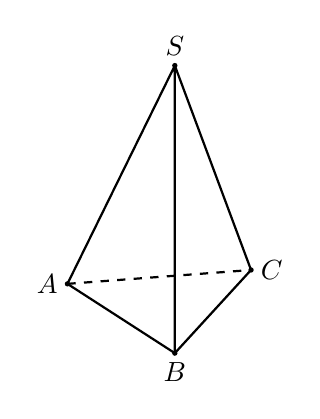
\begin{tikzpicture}[scale=0.88,>=stealth]
  \coordinate (A) at (0,0);
  \coordinate (B) at (1.55,-1.0);
  \coordinate (C) at (2.65,0.2);
  \coordinate (S) at (1.55,3.15);

  \draw[thick] (A)--(B)--(C);
  \draw[dashed,thick] (A)--(C);
  \draw[thick] (S)--(A) (S)--(B) (S)--(C);
  \fill (A) circle (1.1pt) node[left] {$A$};
  \fill (B) circle (1.1pt) node[below] {$B$};
  \fill (C) circle (1.1pt) node[right] {$C$};
  \fill (S) circle (1.1pt) node[above] {$S$};
\end{tikzpicture}
\end{center}
\nopagebreak[4]
\Needspace{4\baselineskip}
\textbf{解析}
\nopagebreak[4]
\begin{center}% 1986 年广东卷文史类第 6 题：三棱锥
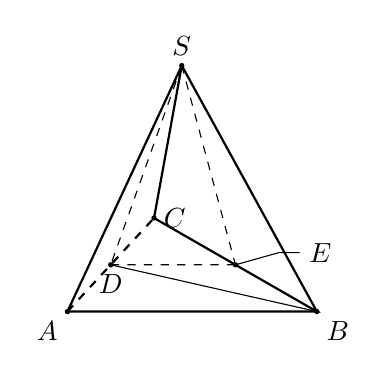
\begin{tikzpicture}[scale=0.88,>=stealth]
  \coordinate (A) at (0,0);
  \coordinate (B) at (3.6,0);
  \coordinate (C) at (1.25,1.35);
  \coordinate (S) at (1.65,3.55);
  \coordinate (D) at (0.625,0.675);
  \coordinate (E) at (2.425,0.675);

\draw[thick] (A)--(B)--(C);
\draw[dashed,thick] (A)--(C);
  \draw[thick] (S)--(A) (S)--(B) (S)--(C);
  \draw[dashed] (S)--(D) (S)--(E) (D)--(E);
  \draw (D)--(B);
  \fill (A) circle (1.1pt) node[below left] {$A$};
  \fill (B) circle (1.1pt) node[below right] {$B$};
  \fill (C) circle (1.1pt) node[right] {$C$};
  \fill (S) circle (1.1pt) node[above] {$S$};
  \fill (D) circle (1.1pt) node[below] {$D$};
  \fill (E) circle (1.1pt);
  \draw (E) -- (3.05,0.85) -- (3.35,0.85) node[right] {$E$};
\end{tikzpicture}
\end{center}
\nopagebreak[4]
\gksubpart{（1）}

\Needspace{5\baselineskip}
在平面 $SAC$ 内作 $SD\perp AC$。由 $SA=SC=b$，$D$ 是 $AC$ 中点，故

\nopagebreak[4]
\[
AD=DC=\frac a2,\qquad
SD=\sqrt{b^2-\frac{a^2}{4}}.
\]

\Needspace{5\baselineskip}
又因 $SAC\perp ABC$，有 $SD\perp ABC$。在底面内

\nopagebreak[4]
\[
BD=\sqrt{a^2+\left(\frac a2\right)^2}
=\frac{\sqrt5}{2}a.
\]

\Needspace{5\baselineskip}
若 $SB$ 与底面所成角为 $\varphi$，则

\nopagebreak[4]
\[
\tan\varphi
=\frac{SD}{BD}
=\frac{\sqrt{20b^2-5a^2}}{5a}.
\]

\gksubpart{（2）}

\Needspace{5\baselineskip}
在平面 $SBC$ 内作 $SE\perp BC$。由于 $SD\perp BC$，截面可取三角形 $SDE$。在底面直角三角形中

\nopagebreak[4]
\[
DE=\frac{\sqrt2}{4}a,
\]

\Needspace{5\baselineskip}
且 $SD\perp DE$。所以截面面积为

\nopagebreak[4]
\[
\frac12SD\cdot DE
=\frac a{16}\sqrt{8b^2-2a^2}.
\]

\gkanswer{答案（1）：$\displaystyle \frac{\sqrt{20b^2-5a^2}}{5a}$}

\gkanswer{答案（2）：$\displaystyle \frac a{16}\sqrt{8b^2-2a^2}$}

\end{answer}
\begin{answer}
\gksolhead{7}{}

\textbf{题目}：

\Needspace{5\baselineskip}
（本题满分 12 分）已知椭圆 $C$ 的直角坐标方程为

\nopagebreak[4]
\[
\frac{x^2}{4}+\frac{y^2}{3}=1,
\]

\Needspace{5\baselineskip}
试确定 $m$ 的取值范围，使得对于直线

\nopagebreak[4]
\[
y=4x+m,
\]

椭圆 $C$ 上有不同的两点关于该直线对称。

\Needspace{4\baselineskip}
\textbf{解析}

\Needspace{5\baselineskip}
设弦所在直线为

\nopagebreak[4]
\[
y=-\frac x4+n.
\]

\Needspace{5\baselineskip}
与椭圆

\nopagebreak[4]
\[
\frac{x^2}{4}+\frac{y^2}{3}=1
\]

\Needspace{5\baselineskip}
联立，交点存在且不同的条件为

\nopagebreak[4]
\[
n^2<\frac{13}{4}.
\]

\Needspace{5\baselineskip}
若交点为 $(x_1,y_1),(x_2,y_2)$，由韦达定理，弦中点为

\nopagebreak[4]
\[
\left(\frac{4n}{13},\frac{12n}{13}\right).
\]

\Needspace{5\baselineskip}
该中点在直线 $y=4x+m$ 上，故

\nopagebreak[4]
\[
\frac{12n}{13}
=4\cdot\frac{4n}{13}+m,
\qquad
m=-\frac{4n}{13}.
\]

\Needspace{5\baselineskip}
由 $|n|<\frac{\sqrt{13}}2$ 得

\nopagebreak[4]
\[
-\frac{2\sqrt{13}}{13}
<m<
\frac{2\sqrt{13}}{13}.
\]

端点对应椭圆与弦相切，只产生一个交点，不能取等号。

\gkanswer{答案：$\displaystyle -\frac{2\sqrt{13}}{13}<m<\frac{2\sqrt{13}}{13}$}

\end{answer}